\documentclass{scirep}

\leftheader{Detektor ATLAS}
\centerheader{Parktikum IV}
\rightheader{Tomáš Derner}

\begin{document}

    \section*{Úkol}

    \begin{enumerate}

        \item Zpracujte přibližně 50 událostí z detektoru ATLAS programem HYPATIA.
        \item Pomocí programu ROOT zobrazte histogram invariantních hmotností pro různě velké statistické soubory.
        \item Identifikujte výrazné píky a přiřaďte je očekávaným částicím.
        \item Zjistěte chybu střední hodnoty invariantní hmotnosti Z bozonu pro různě velké statistické soubory.
        \item Vyneste zjištěné chyby do grafu jako funkci počtu událostí a srovnejte je s očekávanou závislostí.
        \item Interpretujte výsledky statistického testu pro nové částice a rozhodněte, jestli byl učiněn objev.

    \end{enumerate}

    \section*{Teorie}

    V tomto praktiku se zabýváme zpracováním dat z experimentu ATLAS v CERNu, který stál za objevem Higgsova bosonu.
    Právě na detekci Higgsova bosonu společně s Z bosonem se tato úloha zaměřuje.
    Pro práci využijeme program Hypatia, jehož popis lze nalézt ve studijním textu~\cite{pokyny}.

    Zkoumáme rozpadové produkty po čtyřech druzích částic: Higgsovu bosonu, Z bosonu, částici $J / \Psi$ a částici $\Upsilon$, jejichž invariantní hmotnosti jsou uvedeny v tabulce~\ref{tab:particles}.
    Z boson se rozpadá mimo jiné na pár elektron-pozitron nebo na pár mion-antimion, Higgsův boson se rozpadá na pár $Z Z^{(*)}$, přičemž každé $Z$ se poté rozpadá jak je psáno výše, nebo na dvě částice~$\gamma$.
    Rozpad na pár leptonů nebo částic $\gamma$ lze pozorovat i u zbývajících uvedených částic.

    
\begin{table}[h]
    \centering
    \setlength{\tabcolsep}{15pt}
    \begin{tabular}[t]{
l
S[table-format=3.6]
}
    \toprule
    Částice & {Invariantní hmotnost}  \\ \midrule
    $J / \Psi$  & 3.096900 \\
    $\Upsilon$  & 9.4603   \\
    $Z$         & 91.188   \\
    $H$         & 125.09     \\ \bottomrule
\end{tabular}
    \vspace{0pt}
    \caption{Částice, kterých se týká toto praktikum}
    \label{tab:particles}
\end{table}


    Kritérium pro objevení nové částice je $p < \num{3e-7}$, popř. hodnota signifikance $> 5$.

    \section*{Výsledky}

    Pomocí programu Hypatia byly zpracovány události ze dvou souborů, výsledek ukazují histogramy v příloze 1.
    Kvůli velmi nízkému počtu zpracovaných událostí je jediným smysluplným závěrem přítomnost píku odpovídající Z bozonu v histogramu detekce leptonových párů (graf uprostřed nahoře).

    Větší vypovídací hodnotu mají histogramy v příloze 2, které shrnují výsledky zpracování více než tisíc událostí.
    Levý horní graf ukazuje zřejmé píky částic $J / \Psi$ a $\Upsilon$ (podle tabulky~\ref{tab:particles}) a prostřední horní graf opět obsahuje dobře definovaný pík Z bosonu.
    Histogram vpravo obsahuje píky v oblasti $\SI{1000}{GeV/c^2}$ a $\SI{1500}{GeV/c^2}$, které jsou pravděpodobně zapříčiněny vnesením fiktivních dat a neodpovídají známým částicím.

    Histogram detekce fotonových párů(ve třetí řadě vlevo) ukazuje, že i přes značný počet událostí není možné rozlišit pík Higgsova bosonu vůči pozadí (fit píku je dokonce záporný).

    V příloze 3 lze nalézt histogramy zobrazující pík Z bosonu pro různý počet zpracovaných událostí.
    Chyby $s_{\mu}$ určení polohy píků $\mu$ byly přeneseny z grafů do tabulky~\ref{tab:errors} a zobrazeny v závislosti na počtu zpracovaných událostí v grafu na obrázku~\ref{fig:fit_errors}.
    Hodnoty byly proloženy fitem podle rovnice
    \[ s_{\mu} = \frac{a}{\sqrt{N}},~~~ a = \num{3.8 \pm 0.6}. \]

    
\begin{table}[h]
    \centering
    \setlength{\tabcolsep}{15pt}
    \begin{tabular}[t]{
  S[table-format=4.0]
  S[table-format=1.3]
} \toprule
{$N$} & {$s_{\mu}$} \\ \midrule
   50 &       0.360 \\
  100 &       0.550 \\
  200 &       0.340 \\
  500 &       0.183 \\
 1000 &       0.137 \\
 1647 &       0.112 \\ \bottomrule
\end{tabular}
    \vspace{0pt}
    \caption{Závislost hodnoty chyby pozice píku Z bozonu na počtu měření}
    \label{tab:errors}
\end{table}

    
\begin{figure}[h!]
    \centering
    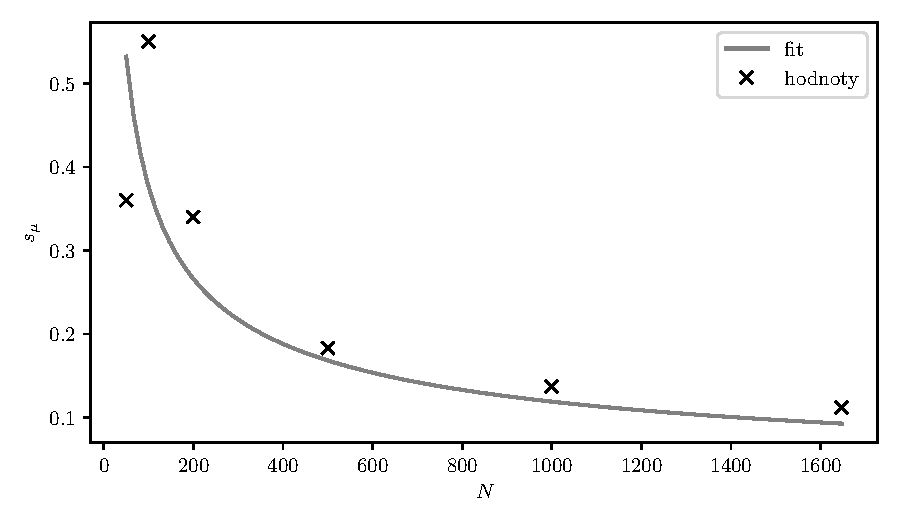
\includegraphics{fit_errors.pdf}
    \vspace{0pt}
    \caption{Závislost hodnoty chyby pozice píku Z bozonu na počtu měření}
    \label{fig:fit_errors}
\end{figure}


    Příloha 4 ukazuje grafy objevování nových částic.
    Ačkoliv v histogramu detekce párů elektronů ($p \approx \num{2e-6}$) a párů fotonů (pík není výrazný) nedosahuje hodnota $p$ a signifikance potřebných hodnot pro objev nové částice v oblasti $\SI{1000}{GeV/c^2}$, hodnota $p = \num{2e-10}$ v grafu detekce párů mionů dostačuje k objevu.
    V oblasti $\SI{1500}{GeV/c^2}$ je nejzřetelnější pík v histogramu detekce párů fotonů, ale jeho hodnota $p \approx \num{4e-4}$ nestačí k objevu.


    \section*{Diskuse}
    Vzhledem ke značně teoretickému rázu úlohy byla diskuse provedena vždy v odpovídající sekci výsledků zpracování.

    \section*{Závěr}
    Bylo provedeno zpracování událostí ze dvou souborů (asi 95 událostí) v programu Hypatia.
    Výsledné histogramy byly diskutovány.
    Průběh závislosti hodnoty chyby polohy píku Z bosonu na počtu měření uspokojivě popisuje závislost
    \[ s_{\mu} = \frac{a}{\sqrt{N}},~~~ a = \num{3.8 \pm 0.6}. \]
    Došlo k objevu částice v oblasti $\SI{1500}{GeV/c^2}$ v histogramu detekce párů mionů ($p = \num{2e-10}$).

    \begin{thebibliography}{}

        \bibitem{pokyny}
        Pokyny k měření ``Objevování částic v detektoru ATLAS v CERN'', dostupné z\\ \url{https://physics.mff.cuni.cz/vyuka/zfp/_media/zadani/texty/txt_401.pdf}, 4.\,12.\,2019

    \end{thebibliography}

\end{document}